\documentclass{article}
\usepackage{listings}
\usepackage{graphicx}
\usepackage{float}
 
\floatstyle{ruled}
\newfloat{program}{thp}{lop}
\floatname{program}{Snippet}


\begin{document}

\title{Project Report - Limited Static Type Checking for JavaScript}
\author{Huascar A. Sanchez \and Tim Disney}

\maketitle

\lstset{showstringspaces=false}

\begin{abstract}
Implementations of static type checkers are available. However, they only worked
for a subset of JavaScript. In this report we explored an alternative that could 
parse full JavaScript code. We called this alternative JScheck. JScheck is a static 
type checker for prototype-based objects in JavaScript. In other words, JSCheck will 
completely ignored things like strings and numbers. 

We study the type checking problem given the definitions studied in class. A set of
changes were made to the HJS parsing library to recognize type annotations in 
JavaScript code. Then, we implemented the major components of JScheck: Type Extractor
and Type Checker. Both components complement each other. The Type Extractor is 
responsible for finding all the JavaScript object types that have been defined. The 
Type Checker is responsible for finding all functions that have been type annotated. 
The result of these functions' invocation indicates if the JavaScript is well typed. 
The main rationale is to prevent the occurrence of errors during program execution. 
\end{abstract}

\section{Introduction}
In the construction of software it is generally cheaper to 
catch programming errors earlier in the development cycle. One common method 
to catch errors is static type checking which can
check the type consistency of the program before it is even
run. If the code has any type violations the type checker will 
find them and alert the programmer.

For example, in strongly typed languages like Java it is impossible 
to invoke a method which has not been defined for a class (unless reflection is used).
The compiler will immediately complain and prevent the program from compiling. However, 
in languages like JavaScript, this kind of error will not be discovered until runtime.

Adding static type checking to a dynamic language like JavaScript is a 
challenge, especially since objects can be modified at runtime. Given this challenge, 
we have implemented a static type checker, called JSCheck, for user-defined objects 
in JavaScript. The scope of JSCheck is limited to properties on an object's
prototype. In other words, we are completely ignoring type checking of the built in types
such as strings and numbers. The whole idea, as Luca Cardelli said \cite{typesystems}, 
is to prevent the occurrence of errors during program execution. 

The rest of this paper is divided as follows. Section (\ref{sec:types}) gives an overview
of how user-defined types work in JavaScript, section (\ref{sec:implementation}) 
will discuss the design and implementation choices that were made through the development 
of JSCheck, related work will be discussed in (\ref{sec:related}), and future work
and conclusions in Sections (\ref{sec:future}) and (\ref{sec:conclusion}).


\section{Types in JavaScript}
\label{sec:types}
User-defined types in JavaScript can be written in a variety of styles and forms. The form
that we considered in the scope of this project is object creation using 
constructor functions and prototype modification.

\begin{program}[here]
\begin{verbatim}
function Dog(){
  // ..
}

Dog.prototype.getName = function(){
  //..
}

Dog.prototype.bark = function(){
  //..
}

var mydog = new Dog();
\end{verbatim}
\caption{Checking Types in JavaScript}
\label{fig:object}
\end{program}
\pagebreak

For example, in Snippet \ref{fig:object} we defined a {\tt Dog} type
which has two methods, {\tt getName} and {\tt bark} which are added to the {\tt Dog}
prototype. New ``instances'' of the {\tt Dog} type can be created with the {\tt new}
keyword.

There are other ways of creating objects including using object literal notation
and assigning methods directly to fields of an existing object. Due to time constraints,
we opted to not include them in the scope of JSCheck.

To enable JSCheck to check the usages of an object we added the comment type annotation
to the JavaScript language as seen in Snippet \ref{fig:check}. In
this example the {\tt fido} parameter has been annotated with the {\tt Dog}
type in the {\tt //\#} comment. JSCheck will then check that all usages of
the {\tt fido} parameter conforms to the definition of the {\tt Dog} type.

\begin{program}[here]
\begin{verbatim}
//# @type Dog fido
function useDog(fido) {
  fido.bark();
}

var mydog = new Dog();
useDog(mydog);
\end{verbatim}
\caption{Type Checking}
\label{fig:check}
\end{program}
\pagebreak

\section{Implementation}
\label{sec:implementation}
JSCheck is implemented in Haskell. We were originally considering defining a 
subset of JavaScript to ease the burden of creating a parser for JavaScript. 
However we found a Haskell library called HJS \cite{hjsLibrary} 
which implements a full parser for JavaScript (ECMAScript 3rd edition plus 
some additions from JavaScript 1.5). We needed to make a few modifications to
HJS in order to pick up the type annotations. This greatly simplified much of
the implementation effort of JSCheck.

Figure \ref{fig:jscheckway} shows in general terms how JSCheck works. JSCheck takes 
in a JavaScript source file and runs
it through a modified version of the HJS parser. This produces an abstract syntax tree
(AST) which is then fed into a type extractor function which finds all the JavaScript 
object types that
have been defined. The output of this function is a list of types 
(type name and all associated fields)
which is given to a type checker function along with the original AST. The
checker function finds all functions that have been annotated with our special
type comments and checks all usages of typed parameters against the extracted types.
The final 
output will be a boolean which represents if the code is well-typed or not. 

\begin{figure}[here]
  \begin{center}
    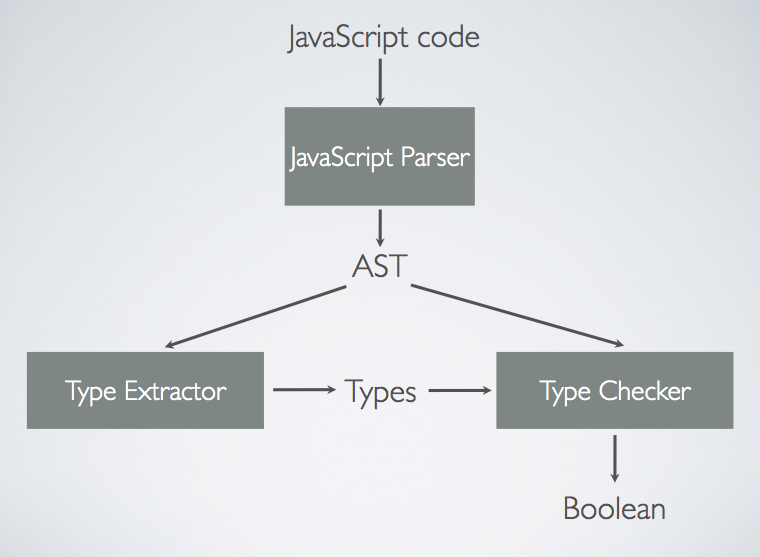
\includegraphics[scale=0.4]{blockdiagram.png}
  \end{center}
  \caption{Type Checking - the JSCheck way}
  \label{fig:jscheckway}
\end{figure}
\pagebreak

Because of the dynamic nature of JavaScript our implementation is both unsound 
and incomplete. It is unsound because methods could be added to the object at
runtime. So, even though the checker may find a usage of an unknown field, that field
might actually be defined. It is incomplete because fields could also be removed
from an object at runtime. The JavaScript program could be accessing non-existent 
fields even though the checker thought they were there.


\section{Testing of the JScheck}
\label{sec:testing}

JScheck went through an exhaustive testing, i.e., functional and unit testing. 
To illustrate the type of code that can be reviewed by JScheck, we created a demo 
page, which is found online at {\tt http://www.hsanchez.net/demo.html}. In this page, 
there is some JavaScript code (See code \ref{fig:demo}) that will get executed every 
time you refresh the browser. JScheck was utilized to determine, at compile time, if 
this code was well-typed. The results showed this code was well-typed.

\begin{program}
\begin{verbatim}
function Guitar(name, color) {
  this.name = name;
  this.color = color;
  this.strings = ['E', 'A', 'D', 'G', 'B', 'e'];
  this.price = 0;
  this.currency = "USD"
}

Guitar.prototype.print = function() {
   var cPrice    = this.price;
   var cCurrency = this.currency;  
   return '<br />' + 'This guitar is ' +
   this.color +
   ', it has ' + this.strings.length + ' strings' +
   ' and it costs ' + cPrice + ' ' + cCurrency;
}

Guitar.prototype.tune = function(newStrings) {
  this.strings = newStrings;
}

var myChords = new Array();
myChords[0] = "DM7";
myChords[1] = "DM9";
myChords[2] = "DM4"; 
Guitar.prototype.play = function() {
  var randomnumber=Math.floor(Math.random()*3)
  return myChords[randomnumber] + " chord was played.";
}
 
Guitar.prototype.update = function (newPrice, newCurrency) {
  this.price    = newPrice;
  this.currency = newCurrency;
}

Guitar.prototype.paint = function (newColor) {
  this.color    = newColor;
}


//# @type Guitar guitar
function describe(guitar) {
  return guitar.print();
}
 
//# @type Guitar guitar
function playTune(guitar){
   return guitar.play();   
}
\end{verbatim}
\caption{JavaScript code to be type-checked}
\label{fig:demo}
\end{program}
\pagebreak


The above JavaScript code, contained in a file called demo.js), was tested by running
a function similar to the one in \ref{fig:functional}. This function takes our demo.js 
file as an input, and then it parses it. The result of this parsing is an AST. This AST 
is then fed to the checker and extractor functions. The result of these functions' invocation 
will tell us whether the code in the demo.js is well-typed.


\begin{program}
\begin{verbatim}    
check_demo_file = do
  s <- readFile "testfiles/demo.js"
  parse_fail s (\p -> if check_now p (runExtractor p)
                        then assertFailure "should have failed the type check" 
                        else assertBool "passed correctly" True)
\end{verbatim}
\caption{Type Checking of Demo.js}
\label{fig:functional}
\end{program}
\pagebreak


\section{Related Work}
\label{sec:related}
Other work has been done to add various forms of static type checking to dynamic
languages like JavaScript. Anderson {\em et al.}
\cite{typeinferenceforjavascriptEcoop, typecheckingforjavascript} had a series of papers
on adding type inference and type checking to a JavaScript subset called $JS_0$. Austin
and Sadowski \cite{fwjsStruct} implemented type checking for another subset of JavaScript called 
Featherweight JavaScript. While the techniques used by both these groups can catch 
many more type errors than JSCheck, 
they also only work for a JavaScript subset while JSCheck can parse full JavaScript code.

There has also been work done adding static typing to other dynamic languages. Furr {\em et al.}
\cite{typecheckingruby} created a tool called DRuby that adds static type inference to
the Ruby language. They also do not use a language subset and can check real Ruby code.

Google has a tool for checking JavaScript called the Closure 
compiler \cite{closureCompiler}. While this tool is mainly focused on minifying
and optimizing JavaScript, it can also do some type checking. It uses type
annotations in comments which is similar to what JSCheck uses.

\section{Future Work}
\label{sec:future}
There are several areas where JSCheck could be expanded. The messages that are displayed
to the user are currently very primitive. JSCheck will only display ``True'' if the
input code is well-typed or ``False'' if it is ill-typed. For this to be a truly useful tool
it would be highly desirable to display the line numbers where type errors were found.

JSCheck could also be extended to understand more forms of object creation. Currently
only constructor function and prototype modification are supported but many other forms
are in common use.

Other future work could include extending the type consistency checks for other elements 
of the language, such as usages of built in types such as strings and numbers.

\section{Conclusion}
\label{sec:conclusion}
Type errors are a frustrating part of developing software in dynamic languages.
We have developed a static type checker for prototype based objects in JavaScript which
can help ease that pain.
By using JSCheck and adding a few type annotations a developer is be able to catch many
type errors before ever running the program. 

All source code for JSCheck is publicly available and can be found online at
{\tt http://github.com/disnet/jscheck}.

\bibliographystyle{abbrv}
\bibliography{report}

\end{document}



